% \documentclass{article}
% \usepackage{xeCJK, fontspec, xunicode, xltxtra}  
% \setCJKmainfont{Hiragino Sans GB}  

% \title{Title}
% \author{}

% \begin{document}

% \maketitle{}

% \section{Introduction}

% This is where you will write your content. 在这里写上内容。

% \end{document


% \documentclass{article}  
% \title{My first Latex document} 
% \author{Yingshan Li} 
% \date{8/26/2018} 
% \begin{document} 
% \maketitle 

% Hello world! 

% \end{document}














\documentclass{article}  

\usepackage{xeCJK, fontspec, xunicode, xltxtra}  
\usepackage{subcaption} % 子标题
\usepackage{cite}
\setCJKmainfont{Hiragino Sans GB}  

\title{My first Latex document} 
\author{Yingshan Li} 
\date{8/26/2018} 
\begin{document} 
\maketitle 
\tableofcontents 

% \section{} 
% \subsection{} 
% \subsubsection{}

\paragraph{} 
dsfsdfds
\subparagraph{} 
sfdsfsd
% \subsubparagraph{}
fsfdsfs

Einstein 's $E=mc^2$.   %行内公式
\[ E=mc^2. \]   %行间公式 自动居中

%插入多个公式
\begin{displaymath} 
S_{n+1} = S_{n} + S_{n},  
S_{n}=1=2^{n} 
\end{displaymath}


%对行间公式进行编号 全文顺序编号的
\begin{equation} 
E=mc^2 
\textbf{哈佛}
\end{equation}
\begin{equation} 
E=mc^2 
\end{equation}


%行内模式
$E=mc^2$ 
%行间模式
$$E=mc^2$$

\begin{equation} 
E=mc^2 
\end{equation}
\begin{equation} 
E=mc^2 
\end{equation}


%换行
Hello world! \\
vgdff \\
dsfsdfds

%上下标
$f^{gdf}$ \\
$v_{dgd}$

%开方
$\sqrt{n}$
$\sqrt[m]{n}$

%累计求和
$\sum_{i=m}^{n}$

%累计求积
$\prod_{i=m}^{n}$


%积分
$\int_{i=m}^n$


%向量
$\vec {a}$\\
$\overrightarrow{AB}$

%省略号
$a+b+\cdots+z$

%大括号
$\underbrace{a+b+\cdots+z}_{26}$

%横杠
$\overline{text+di}_{f}$

{f}
fsfdsfsffff

dfsdgsg\\

但是咕咚咕咚广东省高考的髋关节烤地瓜烤地瓜\\

%无序列表
\begin{itemize}
	\item one
	\item two
\end{itemize}

%有序列表
\begin{enumerate}
	\item one
	\item two
\end{enumerate}
	

%处理参考文献

\section{Greetings} 
\label{sec:greetings}   Hello!   
\section{Referencing}   
I greeted in {section~\ref{sec:greetings}}.



\begin{figure}
    \centering
    \begin{minipage}[c]{0.48\textwidth}
        \centering
        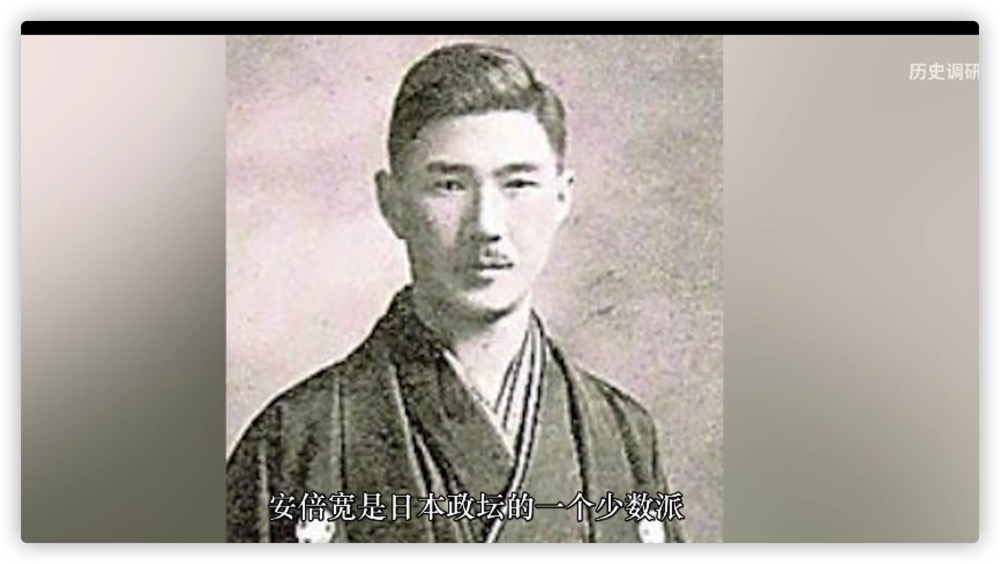
\includegraphics[height=0.2\textheight]{1}
        \subcaption{一只猫}
    \end{minipage}
    \begin{minipage}[c]{0.48\textwidth}
        \centering
        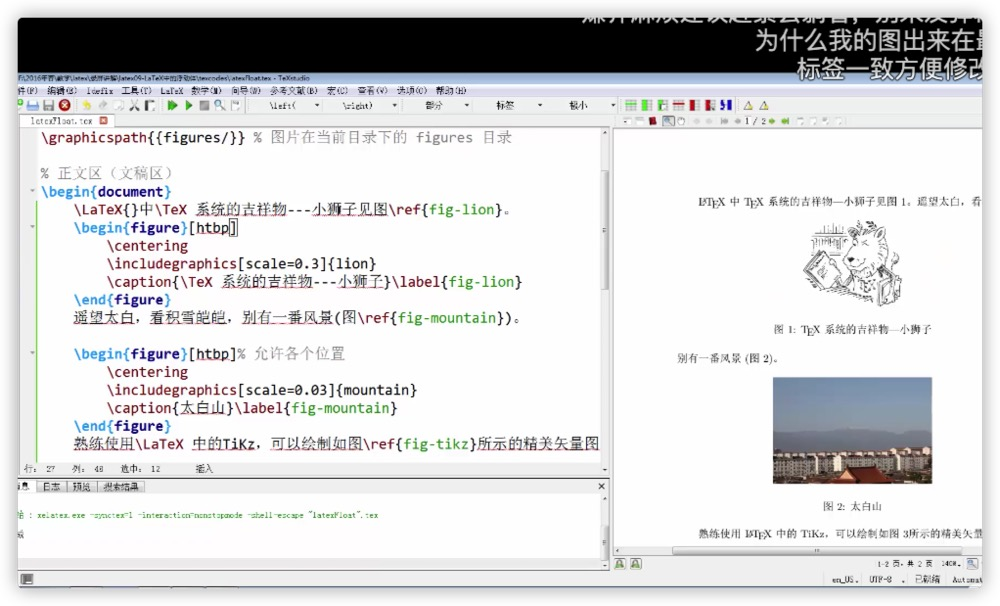
\includegraphics[height=0.2\textheight]{2}
        \subcaption{电路图}
    \end{minipage}
    \caption{多图并排示例}
\end{figure}




hhvjhvjkbjkbkj\cite{Wille1982}hfhjj




%\bibliographystyle{plain}
\bibliography{ref}






























\end{document}


